\documentclass[a4paper,11pt]{report}
\usepackage{chuan_math_gkt}
\usetikzlibrary{angles,quotes,intersections,patterns,decorations.pathreplacing}
\chuanexamsetup

\begin{document}
\examfontsize

\examsecret{绝密$\bigstar$启用前}

\examtitle{2021年普通高等学校招生全国统一考试（新高考II卷）}{数\quad 学}

\noticetitle
\begin{examnotice}
\item 答卷前，考生务必将自己的姓名、准考证号填写在答题卡上. 
\item 回答选择题时，选出每小题的答案后，用铅笔把答题卡上对应题目的答案标号涂黑. 如需改动，用橡皮擦干净后，再选涂其他答案标号. 回答非选择题时，将答案写在答题卡上. 写在本试卷上无效. 
\item 考试结束后，将本试卷和答题卡一并交回. 
\end{examnotice}

\examsection{一、选择题：本题共8小题，每小题5分，共40分. 在每小题给出的四个选项中，只有一项是符合题目要求的.}
\begin{examquestions}

\item 复数 $\dfrac{2-\mathrm{i}}{1-3\mathrm{i}}$ 在复平面内对应点所在的象限为
\fourchoices{第一象限}{第二象限}{第三象限}{第四象限}

\item 设集合 $U=\{1,2,3,4,5,6\}$，$A=\{1,3,6\}$，$B=\{2,3,4\}$，则 $A\cap(\complement_U B)=$
\fourchoices{$\{3\}$}{$\{1,6\}$}{$\{5,6\}$}{$\{1,3\}$}

\item 抛物线 $y^2=2px(p>0)$ 的焦点到直线 $y=x+1$ 的距离为 $\sqrt2$，则 $p=$
\fourchoices{$1$}{$2$}{$2\sqrt2$}{$4$}

\item 北斗三号全球卫星导航系统是我国航天事业的重要成果. 在卫星导航系统中，地球静止同步卫星的轨道位于地球赤道所在平面，轨道高度为 $36000\,\mathrm{km}$（轨道高度是指卫星到地球表面的距离）. 将地球看作是一个球心为 $O$，半径 $r$ 为 $6400\,\mathrm{km}$ 的球，其上点 $A$ 的纬度是指 $OA$ 与赤道平面所成角的度数. 地球表面上能直接观测到一颗地球静止同步轨道卫星点的纬度最大值为 $\alpha$，记卫星信号覆盖地球表面的表面积为 $S=2\pi r^2(1-\cos\alpha)$（单位：$\mathrm{km}^2$），则 $S$ 占地球表面积的百分比约为
\fourchoices{$26\%$}{$34\%$}{$42\%$}{$50\%$}

\item 正四棱台上、下底面的边长分别为 $2,4$，侧棱长为 $2$，则其体积为
\fourchoices
{$20+12\sqrt3$}
{$28\sqrt2$}
{\tallchoice{$\dfrac{56}{3}$}}
{\tallchoice{$\dfrac{28\sqrt2}{3}$}}

\item 某物理量的测量结果服从正态分布 $N(10,\sigma^2)$，下列结论中不正确的是
\onechoices
{$\sigma$ 越小，该物理量在一次测量中在 $(9.9,10.1)$ 的概率越大}
{$\sigma$ 越小，该物理量在一次测量中大于 $10$ 的概率为 $0.5$}
{$\sigma$ 越小，该物理量在一次测量中小于 $9.99$ 与大于 $10.01$ 的概率相等}
{$\sigma$ 越小，该物理量在一次测量中落在 $(9.9,10.2)$ 与落在 $(10,10.3)$ 的概率相等}

\item 已知 $a=\log_5 2$，$b=\log_8 3$，$c=\dfrac12$，则下列判断正确的是
\fourchoices{$c<b<a$}{$b<a<c$}{$a<c<b$}{$a<b<c$}

\item 已知函数 $f(x)$ 的定义域为 $\mathbb R$，$f(x+2)$ 为偶函数，$f(2x+1)$ 为奇函数，则
\fourchoices{\tallchoice{$f\left(-\dfrac12\right)=0$}}{$f(-1)=0$}{$f(2)=0$}{$f(4)=0$}

\end{examquestions}

\examsection{二、选择题：本题共4小题，每小题5分，共20分. 在每小题给出的选项中，有多项符合题目要求. 全部选对的得5分，部分选对的得2分，有选错的得0分.}
\begin{examquestions}[start=9]

\item 下列统计量中，能度量样本 $x_1,x_2,\cdots,x_n$ 的离散程度的是
\twochoices
{样本 $x_1,x_2,\cdots,x_n$ 的标准差}
{样本 $x_1,x_2,\cdots,x_n$ 的中位数}
{样本 $x_1,x_2,\cdots,x_n$ 的极差}
{样本 $x_1,x_2,\cdots,x_n$ 的平均数}

\item 如图，在正方体中，$O$ 为底面的中心，$P$ 为所在棱的中点，$M,N$ 为正方体的顶点. 则满足 $MN\perp OP$ 的是
\graphchoicesoneline
{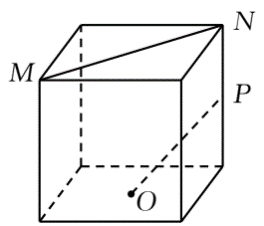
\includegraphics[width=2.5cm]{figures/2021_xgk2_image48.png}}
{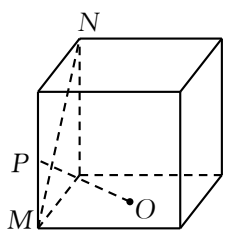
\includegraphics[width=2.3cm]{figures/2021_xgk2_image49.png}}
{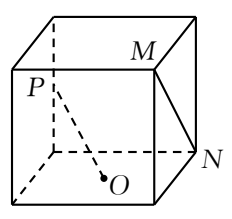
\includegraphics[width=2.3cm]{figures/2021_xgk2_image50.png}}
{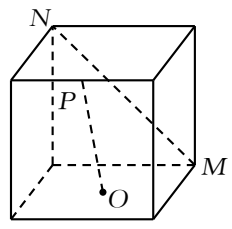
\includegraphics[width=2.3cm]{figures/2021_xgk2_image51.png}}

\item 已知直线 $l:ax+by-r^2=0$ 与圆 $C:x^2+y^2=r^2$，点 $A(a,b)$，则下列说法正确的是
\onechoices
{若点 $A$ 在圆 $C$ 上，则直线 $l$ 与圆 $C$ 相切}
{若点 $A$ 在圆 $C$ 内，则直线 $l$ 与圆 $C$ 相离}
{若点 $A$ 在圆 $C$ 外，则直线 $l$ 与圆 $C$ 相离}
{若点 $A$ 在直线 $l$ 上，则直线 $l$ 与圆 $C$ 相切}

\item 设正整数 $n=a_0\cdot2^0+a_1\cdot2+\cdots+a_{k-1}\cdot2^{k-1}+a_k\cdot2^k$，其中 $a_i\in\{0,1\}$，记 $\omega(n)=a_0+a_1+\cdots+a_k$. 则
\twochoices{$\omega(2n)=\omega(n)$}{$\omega(2n+3)=\omega(n)+1$}{$\omega(8n+5)=\omega(4n+3)$}{$\omega(2^n-1)=n$}

\end{examquestions}
\newpage
\examsection{三、填空题：本题共4小题，每小题5分，共20分.}
\begin{examquestions}[start=13]

\item 已知双曲线 $\dfrac{x^2}{a^2}-\dfrac{y^2}{b^2}=1(a>0,b>0)$ 的离心率为 $2$，则该双曲线的渐近线方程为 \blank.

\item 写出一个同时具有下列性质 \gktcircled{1}\gktcircled{2}\gktcircled{3} 的函数 $f(x)$：\blank.

\gktcircled{1} $f(x_1x_2)=f(x_1)f(x_2)$；\gktcircled{2} 当 $x\in(0,+\infty)$ 时，$f'(x)>0$；\gktcircled{3} $f'(x)$ 是奇函数.

\item 已知向量 $\vec a+\vec b+\vec c=\vec0$，$|\vec a|=1$，$|\vec b|=|\vec c|=2$，则 $\vec a\cdot\vec b+\vec b\cdot\vec c+\vec c\cdot\vec a=$ \blank.

\item 已知函数 $f(x)=|e^x-1|$，$x_1<0$，$x_2>0$，函数 $f(x)$ 的图象在点 $A(x_1,f(x_1))$ 和点 $B(x_2,f(x_2))$ 的两条切线互相垂直，且分别交 $y$ 轴于 $M,N$ 两点，则 $\dfrac{|AM|}{|BN|}$ 取值范围是 \blank.

\end{examquestions}

\examsection{四、解答题：本题共6小题，共70分. 解答应写出文字说明、证明过程或演算步骤.}
\begin{examanswers}[start=17]

\item（10分）

记 $S_n$ 是公差不为 $0$ 的等差数列 $\{a_n\}$ 的前 $n$ 项和，若 $a_3=S_5$，$a_2a_4=S_4$.

\subq{（1）}{求数列 $\{a_n\}$ 的通项公式 $a_n$；}

\subq{（2）}{求使 $S_n>a_n$ 成立的 $n$ 的最小值.}

\item（12分）

在 $\triangle ABC$ 中，角 $A,B,C$ 所对的边长分别为 $a,b,c$，$b=a+1$，$c=a+2$.

\subq{（1）}{若 $2\sin C=3\sin A$，求 $\triangle ABC$ 的面积；}

\subq{（2）}{是否存在正整数 $a$，使得 $\triangle ABC$ 为钝角三角形？若存在，求出 $a$ 的值；若不存在，说明理由.}

\item（12分）

在四棱锥 $Q-ABCD$ 中，底面 $ABCD$ 是正方形，若 $AD=2$，$QD=QA=\sqrt5$，$QC=3$.


\noindent\begin{minipage}[t]{0.62\linewidth}
\subq{（1）}{证明：平面 $QAD\perp$ 平面 $ABCD$；}

\subq{（2）}{求二面角 $B-QD-A$ 的平面角的余弦值.}
\end{minipage}\hfill
\begin{minipage}[t]{0.32\linewidth}
\vspace{-1em}
\centering
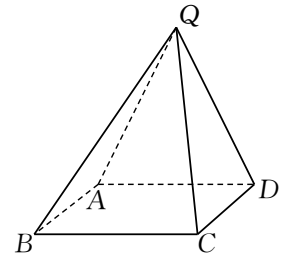
\includegraphics[width=4.5cm]{figures/2021_xgk2_image96.png}
\end{minipage}

\newpage
\item（12分）

已知椭圆 $C$ 的方程为 $\dfrac{x^2}{a^2}+\dfrac{y^2}{b^2}=1(a>b>0)$，右焦点为 $F(\sqrt2,0)$，且离心率为 $\dfrac{\sqrt6}{3}$.

\subq{（1）}{求椭圆 $C$ 的方程；}

\subq{（2）}{设 $M,N$ 是椭圆 $C$ 上的两点，直线 $MN$ 与曲线 $x^2+y^2=b^2(x>0)$ 相切. 证明：$M,N,F$ 三点共线的充要条件是 $|MN|=\sqrt3$.}

\item（12分）

一种微生物群体可以经过自身繁殖不断生存下来，设一个这种微生物为第 $0$ 代，经过一次繁殖后为第 $1$ 代，再经过一次繁殖后为第 $2$ 代 $\ldots$，该微生物每代繁殖的个数是相互独立的且有相同的分布列，设 $X$ 表示 $1$ 个微生物个体繁殖下一代的个数，$P(X=i)=p_i(i=0,1,2,3)$.

\subq{（1）}{已知 $p_0=0.4,p_1=0.3,p_2=0.2,p_3=0.1$，求 $E(X)$；}

\subq{（2）}{设 $p$ 表示该种微生物经过多代繁殖后临近灭绝的概率，$p$ 是关于 $x$ 的方程 $p_0+p_1x+p_2x^2+p_3x^3=x$ 的一个最小正实根，求证：当 $E(X)\leq1$ 时，$p=1$；当 $E(X)>1$ 时，$p<1$；}

\subq{（3）}{根据你的理解说明（2）问结论的实际含义.}

\item（12分）

已知函数 $f(x)=(x-1)e^x-ax^2+b$.

\subq{（1）}{讨论 $f(x)$ 的单调性；}

\subq{（2）}{从下面两个条件中选一个，证明：$f(x)$ 有一个零点.

\gktcircled{1} $\dfrac12<a\leq\dfrac{e^2}{2}$，$b>2a$；

\gktcircled{2} $0<a<\dfrac12$，$b\leq2a$.}

\end{examanswers}

\end{document}